\section{LTC with n-dimension with LTC original}
We conducted two experiments using Motsai's Neblina 
module, a system 
with a Nordic Semiconductor nRF52832 micro-controller, 64~KB of RAM, 
and Bluetooth Low Energy connectivity. Neblina has a 3D 
accelerometer, a 3D gyroscope, a 3D magnetometer, and environmental 
sensors for humidity, temperature and pressure. The platform is 
equipped with sensor fusion algorithms for 3D orientation tracking and 
a machine learning engine for complex motion analysis and motion 
pattern recognition~\cite{sarbishei2016accuracy}. Neblina has a 
battery of 100mAh; at 200~Hz, its average consumption is 2.52~mA when using 
accelerometer and gyroscope sensors but without radio 
transmission, and 3.47~mA with radio transmission, leading to an 
autonomy of 39.7~h without transmission and 28.8~h with transmission. 

\subsection{Experiment 1: validation}

%\todo{(Put a picture of Neblina in a box worn 
%on the wrist)}
\begin{wrapfigure}{R}{3cm}
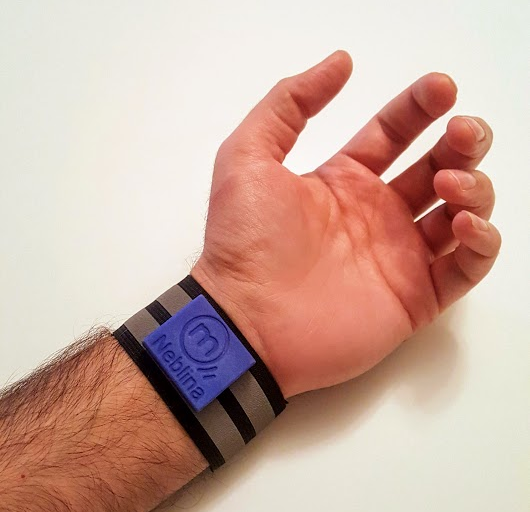
\includegraphics[width=3cm]{figures/neblina-wrist.png}
\caption{Setup with Neblina.}
\label{fig:neblina-wrist}
\end{wrapfigure}
We validated the behavior of our LTC extension on a PC using data 
acquired with Neblina. We collected two 3D accelerometer time-series, a 
short one and a longer one, acquired on two different subjects 
performing biceps curl, with a 50~Hz sampling rate (see 
Figure~\ref{fig:datasets-1}) \TG{Make sure the Figure is aligned with the page, it's not the case}.
In both cases, the subject was wearing 
Neblina on their wrist, as in Figure~\ref{fig:neblina-wrist} \TG{Remove Figure wrapping, it's confusing.}. It should be noted that the longest
time-series also has a higher amplitude, perhaps due to differences between 
subjects.

\begin{figure*}
\centering
\begin{subfigure}{1.2\columnwidth}
\centering
\includegraphics[width=0.3\columnwidth]{figures/5-time-bicep-curl-plot-x.pdf}
\includegraphics[width=0.3\columnwidth]{figures/5-time-bicep-curl-plot-y.pdf}
\includegraphics[width=0.3\columnwidth]{figures/5-time-bicep-curl-plot-z.pdf}
\caption{Short biceps curl$^a$}
\end{subfigure}

{\footnotesize $^a$ Average 
of az data is -7.81mg. It was shifted to 0 so that the graphs can all 
use the same y scale.}

\begin{subfigure}{1.2\columnwidth}
\centering
\includegraphics[width=0.3\columnwidth]{figures/Mohammad-bicep-curl-plot-x.pdf}
\includegraphics[width=0.3\columnwidth]{figures/Mohammad-bicep-curl-plot-y.pdf}
\includegraphics[width=0.3\columnwidth]{figures/Mohammad-bicep-curl-plot-z.pdf}
\caption{Long biceps curl}
\end{subfigure}

\caption{Time-series used in Experiment 1}
\label{fig:datasets-1}
\end{figure*}

We compressed the time-series with various values of $\epsilon$, using 
our 2D (x and y) and 3D (x, y and z) implementations of LTC. On 
Neblina, the raw uncalibrated accelerometer data corresponds to errors 
around 20~mg (1~g is 9.8~m/s$^2$). We used a 
laptop computer with 16~GB of RAM, an Intel i5-3210M CPU @ 2.50GHz 
$\times$ 4, and Linux Fedora 27. We measured memory consumption using 
Valgrind's massif 
tool~\cite{nethercote2006building}, 
and processing time using \texttt{gettimeofday()} from the GNU C 
Library. 

Results are reported in Table~\ref{table:results-validation}. 
As expected, the compression ratio increases with $\epsilon$, and the 
maximum measured error remains lower than $\epsilon$ in all cases. The 
maximum is reached most of the time on these time-series.

\paragraph{Infinity vs Euclidean norms}
The average ratio between the compression ratios obtained
with the infinity and Euclidean norms is 1.03 for 2D data, and 1.06
for 3D data. These ratios are lower than the theoretical values of
$\frac{4}{\pi}$ in 2D and $\frac{6}{\pi}$ in 3D, which are obtained for
random-uniform signals. Unsurprisingly, the infinity norm surpasses the
Euclidean norm in terms of resource consumption. Memory-wise, the
infinity norm requires a constant amount of 80~B, used to store the
intersection of n-balls. The Euclidean norm, however, uses up to 4.7~KB of memory
for the Long time-series in 3D with $\epsilon$=48.8~mg. More importantly,
the amount of required memory increases for longer time-series, and it also increases with larger
values of $\epsilon$. Similar observations are made for the processing
time, with values ranging from 0.4~ms for the simplest time-series and
smallest $\epsilon$, to 41.3~ms for the most complex time-series and
largest~$\epsilon$.
%~ Figure~\ref{fig:memory} shows the memory consumption
%~ of the 3D Euclidean implementation for $\epsilon$=48.8~mg: peaks appear
%~ at the end of long compressed ranges where the signal was $\epsilon$-closed
%~ to the linear approximation.

\paragraph{2D vs 3D}
For a given $\epsilon$, the compression
ratios are always higher in 2D than in 3D. It makes sense since the
probability for the signal to deviate from a straight line
approximation is higher in 3D than it is in 2D. Besides, resource
consumption is higher in 3D than in 2D: for the infinity norm, 3D
consumes 1.4 times more memory than 2D (1.8 times on average for
Euclidean norm), and processing time is 1.35 longer (1.34 on
average for Euclidean norm).

\begin{table}
    \begin{subfigure}{\columnwidth}
    \centering
    \begin{tabular}{l|l|l|l|l}
    \hline
    \rowcolor{headcolor}
                           & \multicolumn{2}{c|}{Infinity} & \multicolumn{2}{c}{Euclidean}\\
    \rowcolor{headcolor}
    $\epsilon$  (mg)          & 48.8         & 34.5       & 48.8       & 34.5 \\
    \hline
    Max error   (mg)          & 48.8         & 34.4       & 48.8       & 34.5 \\
    Compression ratio (\%)    & 79.77        & 72.59      & 77.49      & 70.96\\
    Peak memory   (B)         & 80           & 80         & 688        & 688  \\
    Processing time (ms)      & 0.101        & 0.094      & 0.456      & 0.406\\ \hline
    \end{tabular}
    \caption{Short biceps curl (2D)}
    \end{subfigure}\\
    \begin{subfigure}{\columnwidth}
    \centering
    \begin{tabular}{l|l|l|l|l}
    \hline
    \rowcolor{headcolor}
                   & \multicolumn{2}{c|}{Infinity} & \multicolumn{2}{c}{Euclidean} \\
    \rowcolor{headcolor}
    $\epsilon$ (mg)            & 48.8        & 34.5       & 48.8        & 34.5    \\
    \hline
    Max error  (mg)            & 48.8        & 34.5       & 48.8        & 34.5             \\
    Compression ratio (\%)     & 77.46       & 70.98      & 75.77       & 68.81           \\
    Peak memory  (B)           & 80          & 80         & 2512        & 2608             \\
    Processing time (ms)       & 6.06        & 5.84       & 33.84       & 31.07           \\ \hline
    \end{tabular}
    \caption{Long biceps curl (2D)}
    \end{subfigure}\\
    \begin{subfigure}{\columnwidth}
    \centering
    \begin{tabular}{l|l|l|l|l}
    \hline
    \rowcolor{headcolor}
                           & \multicolumn{2}{c|}{Infinity} & \multicolumn{2}{c}{Euclidean} \\
    \rowcolor{headcolor}
    $\epsilon$ (mg)        & 48.8          & 28.2          & 48.8   & 28.2   \\
    \hline
    Max error  (mg)        & 48.8          & 28.2          & 48.8   & 28.2   \\
    Compression ratio (\%) & 78.14         & 66.39         & 74.39  & 63.13   \\
    Peak memory (B)        & 112           & 112           & 1744   & 784    \\
    Processing time (ms)   & 0.147         & 0.134         & 0.731  & 0.514  \\ \hline
    \end{tabular}
    \caption{Short biceps curl (3D)}
    \end{subfigure}\\
    \begin{subfigure}{\columnwidth}
    \centering
    \begin{tabular}{l|l|l|l|l}
    \hline
    \rowcolor{headcolor}
                              & \multicolumn{2}{c|}{Infinity} & \multicolumn{2}{c}{Euclidean} \\
    \rowcolor{headcolor}
    $\epsilon$ (mg)                & 48.8        & 28.2       & 48.8     & 28.2    \\
    \hline
    Max error  (mg)                & 48.8        & 28.2       & 48.8     & 28.2    \\
    Compression ratio (\%)         & 71.23       & 58.11      & 67.35    & 53.24   \\
    Peak memory (B)                & 112         & 112        & 4752     & 3856    \\
    Processing time (ms)           & 7.87        & 7.22       & 41.29    & 39.04   \\ \hline
    \end{tabular}
    \caption{Long biceps curl (3D)}
    \end{subfigure}
    \caption{Results from Experiment 1}
    \label{table:results-validation}
\end{table}

\begin{figure*}
\centering
\begin{subfigure}{1.2\columnwidth}
\centering
\includegraphics[width=0.3\columnwidth]{./figures/walking-1000-x.pdf}
\includegraphics[width=0.3\columnwidth]{./figures/walking-1000-y.pdf}
\includegraphics[width=0.3\columnwidth]{./figures/walking-1000-z.pdf}
\caption{Walking}
\end{subfigure}
\begin{subfigure}{1.2\columnwidth}
\centering
\includegraphics[width=0.3\columnwidth]{./figures/running-1000-x.pdf}
\includegraphics[width=0.3\columnwidth]{./figures/running-1000-y.pdf}
\includegraphics[width=0.3\columnwidth]{./figures/running-1000-z.pdf}
\caption{Running}
\end{subfigure}
\caption{Time series used in Experiment 2 \vspace*{-0.3cm}}
\label{fig:datasets-2}
\end{figure*}

%~ \begin{figure}
%~ \includegraphics[width=\columnwidth]{./figures/memory-mohammad.pdf}
%~ \caption{Memory usage of 3D Euclidean implementation, long biceps curl time-series, $\epsilon$=48.8~mg.}
%~ \label{fig:memory}
%~ \end{figure}

\subsection{Experiment 2: impact on energy consumption}

We acquired two 3D accelerometer time-series at 200~Hz for two 
activities: walking and running (see Figure~\ref{fig:datasets-2}). In 
both cases, the subject was wearing Neblina on their wrist as in 
Experiment 1. We collected 1,000 data points for each activity, 
corresponding to 5 seconds of activity.

We measured energy consumption associated with the transmission of 
these time-series by ``replaying" the time-series after loading them as 
a byte array in Neblina. We measured the current every 500~ms. We also 
measured the max and average latency resulting from compression.

 Results are reported in Table~\ref{table:results-energy}. For a given
 $\epsilon$ and norm, the compression ratio is larger for walking than
 for running. The ratio of saved energy is relative to the reference
 current of 3.47~mA measured when Neblina transmits data without
 compression. In all cases, activating compression saves energy. The 
 reduction in energy consumption behaves as the compression ratio: it 
 increases with $\epsilon$, it is higher for the infinity norm than for 
 the Euclidean, and it is higher for the walking activity than for 
 running. For a realistic error of $\epsilon$=9.8~mg, the ratio of 
 saved energy with the infinity norm is close to 20\% for the walking 
 activity, which is substantial. Latency is higher for walking 
 than for running, and it is also higher for the Euclidean norm than 
 for the infinity norm. In all cases, the latency remains lower 
 than the 5-ms tolerable latency at 200~Hz, which demonstrates the 
 feasibility of 3D LTC compression.

\begin{table}[]
   \begin{subfigure}{\columnwidth}
   \centering
   \begin{tabular}{l|l|l|l|l|l|l}
   \hline
   \rowcolor{headcolor}
                          & \multicolumn{3}{c|}{Infinity} & \multicolumn{3}{c}{Euclidean} \\
   \rowcolor{headcolor}
   $\epsilon$ (mg)             & 48.8    & 9.8      & 4.9   & 48.8   & 9.8   & 4.9   \\
   \hline
   Max error (mg)              & 48.8    & 9.8      & 4.9   & 48.8   & 9.8   & 4.9   \\
   Compr.      ratio (\%)      & 88.9    & 66.4     & 45.5  & 87.6   & 63.3  & 37.2  \\
   Average (mA)                & 2.64    & 2.79     & 3.02  & 3.10   & 3.02  & 3.13  \\
   Saved energy (\%)           & 23.9    & 19.7     & 13.0  &  10.7  & 13.0  & 9.7   \\
   Max latency ($\mu$s)& 60      & --       & --    & 1530   & --    & --    \\
   Average latency ($\mu$s) & 31 & --       & --    & 145    & --    & --    \\    
   \hline
   \end{tabular}
   \caption{Walking}
   \end{subfigure}
   \begin{subfigure}{\columnwidth}
   \centering
   \begin{tabular}{l|l|l|l|l|l|l}
   \hline
   \rowcolor{headcolor}

                     & \multicolumn{3}{c|}{Infinity} & \multicolumn{3}{c}{Euclidean} \\
    \rowcolor{headcolor}
   $\epsilon$ (mg)        & 48.8       & 9.8      & 4.9       & 48.8      & 9.8    & 4.9    \\
   \hline
   Max error (mg)         & 48.8       & 9.8      & 4.9       & 48.8      & 9.8    & 4.9   \\
   Compr.      ratio (\%) & 68.6       & 25.5     & 9.5       & 64.4      & 19.8   & 5.7   \\
   Average (mA)        & 2.88     & 3.22   & 3.38     & 2.95    & 3.32    & 3.39   \\
   Saved energy (\%)      & 17.0    & 7.2    & 2.5   & 14.9   & 4.3   & 2.2\\
   Max latency ($\mu$s)& 60      & --       & --    & 840   & --    & --    \\
   Average latency ($\mu$s) & 30 & --       & --    & 64    & --    & --    \\    
   \hline
   \end{tabular}
   \caption{Running}
   \end{subfigure}
   \caption{Results from Experiment 2}
   \label{table:results-energy}
\end{table}

\TG{In your conclusion chapter, you should explain what has been implemented
by Motsai on Neblina, this is also a result of your thesis.}